\documentclass{article}

\usepackage{graphicx}
\usepackage{rotating}
\usepackage{amsmath}
\usepackage{amssymb}
\usepackage{fancyhdr}
\usepackage{listings}
%\usepackage{xcolor}
\usepackage{color}
\usepackage{amsfonts}
\usepackage{textcomp}
\usepackage{float}
\usepackage{longtable}
\usepackage[sorting=none]{biblatex}
\usepackage[margin=1in]{geometry}
\usepackage[font={small,it}]{caption}
\usepackage[table,xcdraw]{xcolor}
\usepackage{placeins}
\usepackage{xepersian}





%\DeclareMathOperator*{\btie}{\bowtie}
\addbibresource{bibliography.bib}
\settextfont[Scale=1.2]{B-NAZANIN.TTF}
\setlatintextfont[Scale=1]{Times New Roman}
\renewcommand{\baselinestretch}{1.5}
\pagestyle{fancy}
\fancyhf{}
\rhead{تکلیف تئوری اول درس کامپایلر}
\lhead{\thepage}
\rfoot{علیرضا ابره فروش}
\lfoot{9816603}
\renewcommand{\headrulewidth}{1pt}
\renewcommand{\footrulewidth}{1pt}
%%%%%%%%%%
\lstset
{
    language=[latex]tex,
    basicstyle=\ttfamily,
    commentstyle=\color{black},
    columns=fullflexible,
    keepspaces=true,
    upquote=true,
    showstringspaces=false,
    morestring=[s]\\\%,
    stringstyle=\color{black},
}
%%%%%%%%%%
%beginMatlab
\definecolor{mygreen}{RGB}{28,172,0} % color values Red, Green, Blue
\definecolor{mylilas}{RGB}{170,55,241}
%endMatlab
\begin{document}
%beginMatlab
\lstset{language=Matlab,%
    %basicstyle=\color{red},
    breaklines=true,%
    morekeywords={matlab2tikz},
    keywordstyle=\color{blue},%
    morekeywords=[2]{1}, keywordstyle=[2]{\color{black}},
    identifierstyle=\color{black},%
    stringstyle=\color{mylilas},
    commentstyle=\color{mygreen},%
    showstringspaces=false,%without this there will be a symbol in the places where there is a space
    numbers=left,%
    numberstyle={\tiny \color{black}},% size of the numbers
    numbersep=9pt, % this defines how far the numbers are from the text
    emph=[1]{for,end,break},emphstyle=[1]\color{red}, %some words to emphasise
    %emph=[2]{word1,word2}, emphstyle=[2]{style},    
}
%endMatlab
\begin{titlepage}
\begin{center}

\includegraphics[width=0.4\textwidth]{figures/IUT Logo.png}\\
        
\LARGE
\textbf{دانشگاه صنعتی اصفهان}\\
\textbf{دانشکده مهندسی برق و کامپیوتر}\\
        
\vfill
        
\huge
\textbf{عنوان: تکلیف چهارم درس ریزپردازنده}\\
        
\vfill
        
\LARGE
\textbf{نام و نام خانوادگی: علیرضا ابره فروش}\\
\textbf{شماره دانشجویی: 9816603}\\
\textbf{نیم\,سال تحصیلی: پاییز 1400}\\
\textbf{مدرّس: دکتر عارف کریمی افشار}\\
\end{center}
\end{titlepage}


%\tableofcontents
\newpage


\section{}%1
\subsection{}
خطاهای شناسایی شده توسط تحلیلگر لغوی معمولا دارای ویژگی های زیر هستند:
\begin{itemize}
\item این خطاها زمانی رخ می‌دهند که دنباله ورودی از کاراکترهای معتبر در زبان برنامه‌نویسی مورد نظر تشخیص داده نمی‌شود.
\item این خطاها به طور کلی توسط تحلیلگر لغوی تشخیص داده می‌شوند که در مرحله اول فرایند کامپایل است.
\item این خطاها اغلب به دلیل خطاهای نحوی، مانند کلمات کلیدی یا شناسه‌های نوشتاری نادرست یا کاراکترهای نامعتبر یا نمادها ایجاد می‌شوند.
\end{itemize}

\subsection{}
چهار نمونه مختلف از انواع خطاهای شناسایی شده توسط تحلیل‌گر لغوی، شامل موارد زیر می‌شوند:

\begin{enumerate}
\item کاراکترهای غیرمجاز: این کاراکترها که در زبان برنامه‌نویسی شناخته نشده‌اند، مانند کاراکترهای غیر چاپ‌پذیر یا نویسه‌هایی از زبان‌های دیگر هستند.
\item عدم تطابق نقل قول: این خطا هنگامی رخ می‌دهد که یک متن رشته‌ای به درستی با نقل قول متناظر خاتمه نمی‌یابد. به عنوان مثال، \lr{"Hello، World!} احتمالاً به دلیل عدم وجود دابل کوتیشن پایانی، با خطای لغوی روبرو می‌شود.
\item
\end{enumerate}

\section{}%2

کامپایلر برنامه‌ای است که می تواند یک برنامه از یک زبان (زبان منبع) را بخواند و آن را به یک برنامه معادل به زبان دیگری (زبان هدف) ترجمه کند. نقش مهمی که کامپایلر ایفا می‌کند، گزارش هر نوع خطایی در برنامه‌ی منبع است که در طول فرآیند ترجمه تشخیص داده می‌شود.
\begin{figure}[H]
    \centering
    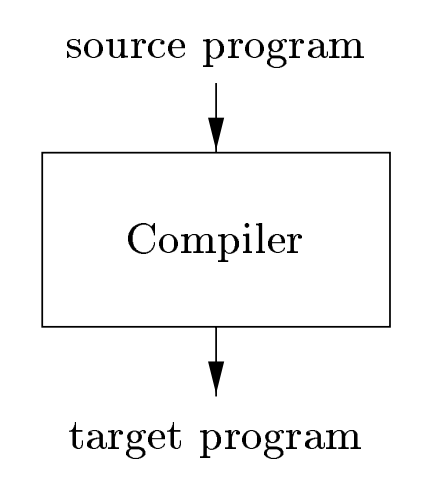
\includegraphics[width=0.25\textwidth]{figures/2a.png}
    \caption
	{}
    \label{fig:fig1}
\end{figure}
یک مترجم (مفسر) نیز یک نوع دیگر از پردازشگر زبان است. به جای تولید یک برنامه هدف به عنوان ترجمه، یک مترجم به نظر می‌رسد که به طور مستقیم عملیات مشخص شده در برنامه‌ی منبع را در ورودی‌هایی تأمین شده توسط کاربر اجرا می‌کند.
\begin{figure}[H]
    \centering
    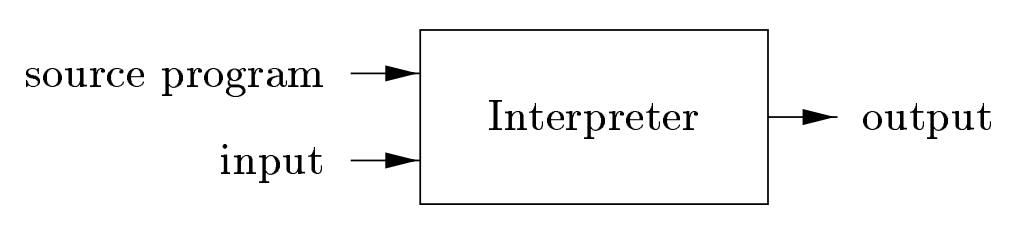
\includegraphics[width=0.5\textwidth]{figures/2b.png}
    \caption
	{}
    \label{fig:fig1}
\end{figure}

\section{}%3
\subsection{}
\begin{latin}
$
\left( \varepsilon \cup \left( 0 \cup 1 \right) ^ {*} 1 \right) \left( 00 \right) ^ {+} \left( 1 \cup 1\left( 0 \cup 1 \right) ^ {*}1 \right) \left( 00 \right) ^ {+} \left( 1 \left( 0 \cup 1 \right) ^ {*} \cup \varepsilon \right)
$
\end{latin}
\subsection{}
\begin{figure}[H]
    \centering
    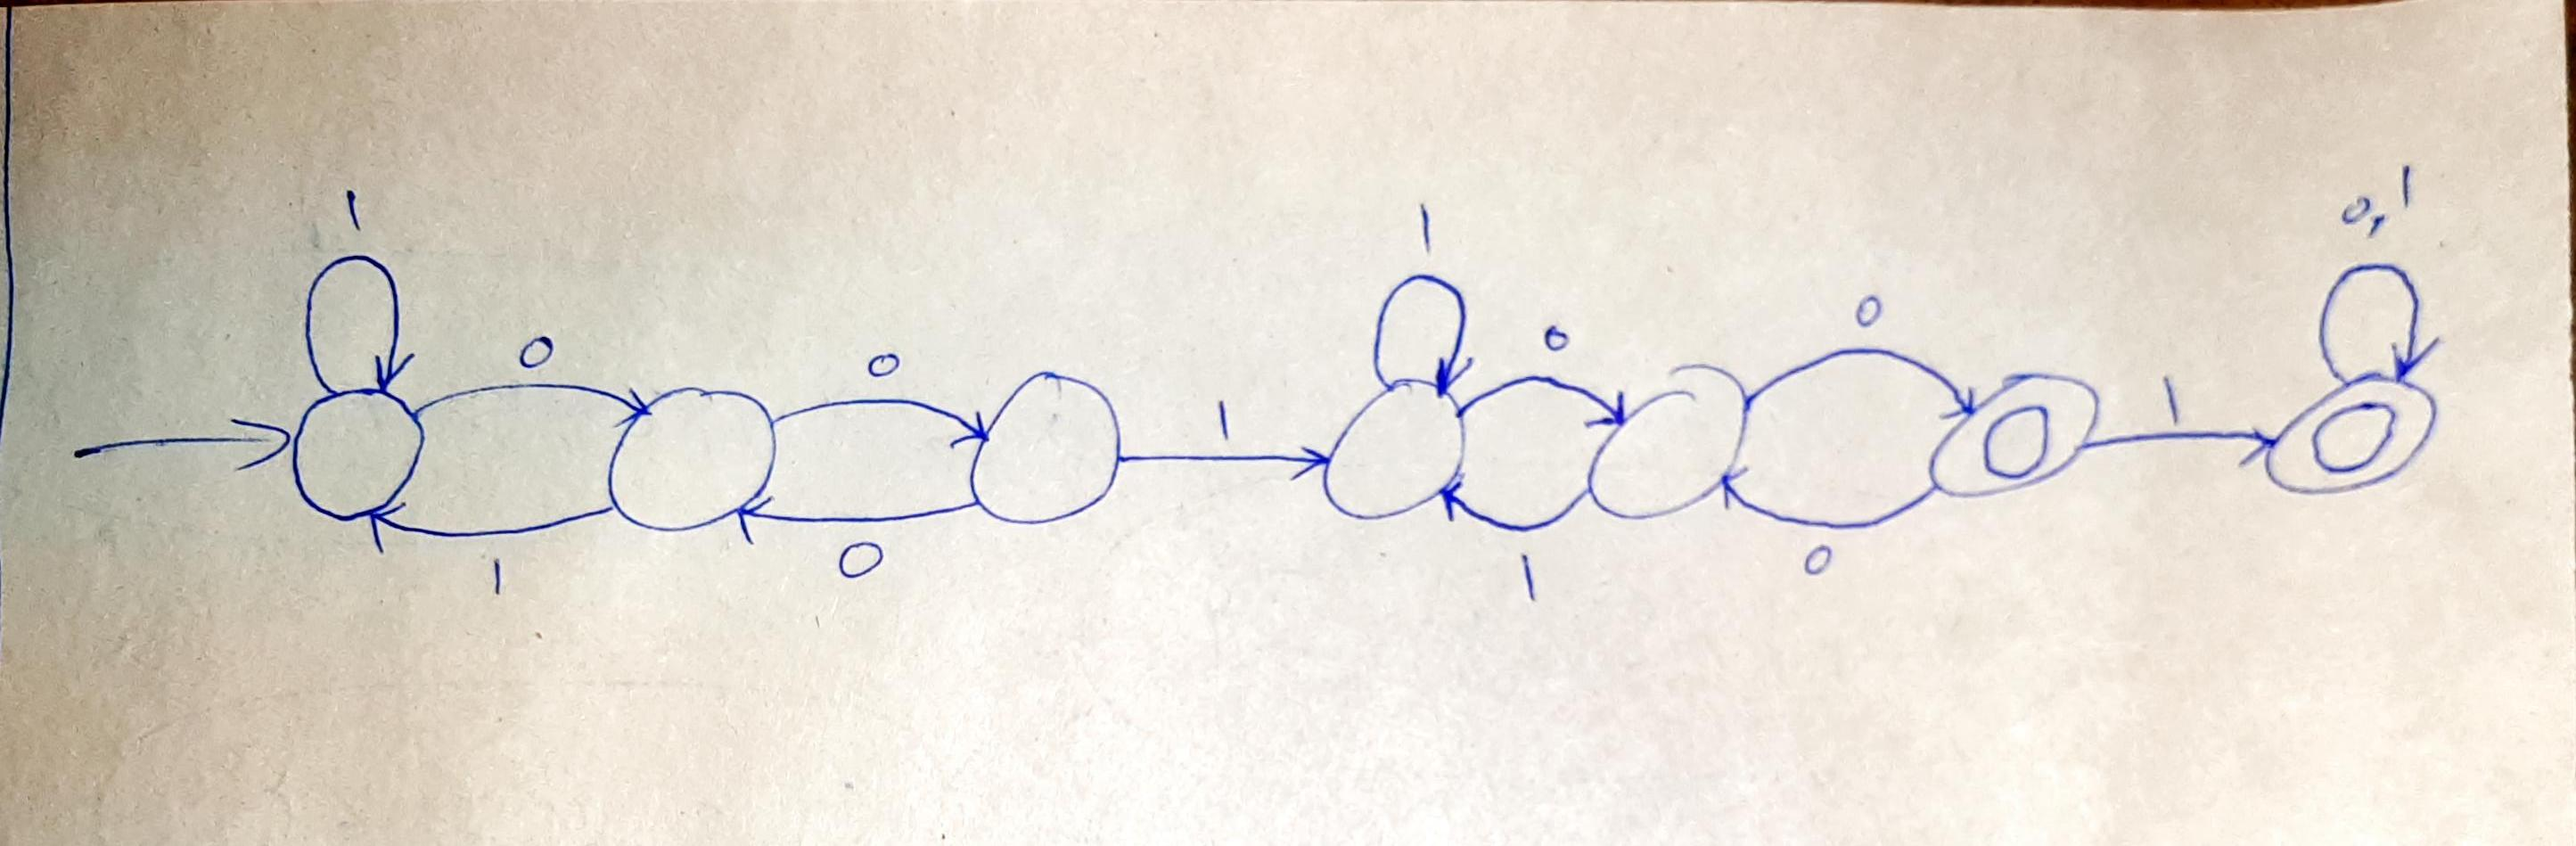
\includegraphics[width=1\textwidth]{figures/3b.jpg}
    \caption
	{}
    \label{fig:fig1}
\end{figure}

\section{}%4
\subsection{الف}
\begin{figure}[H]
    \centering
    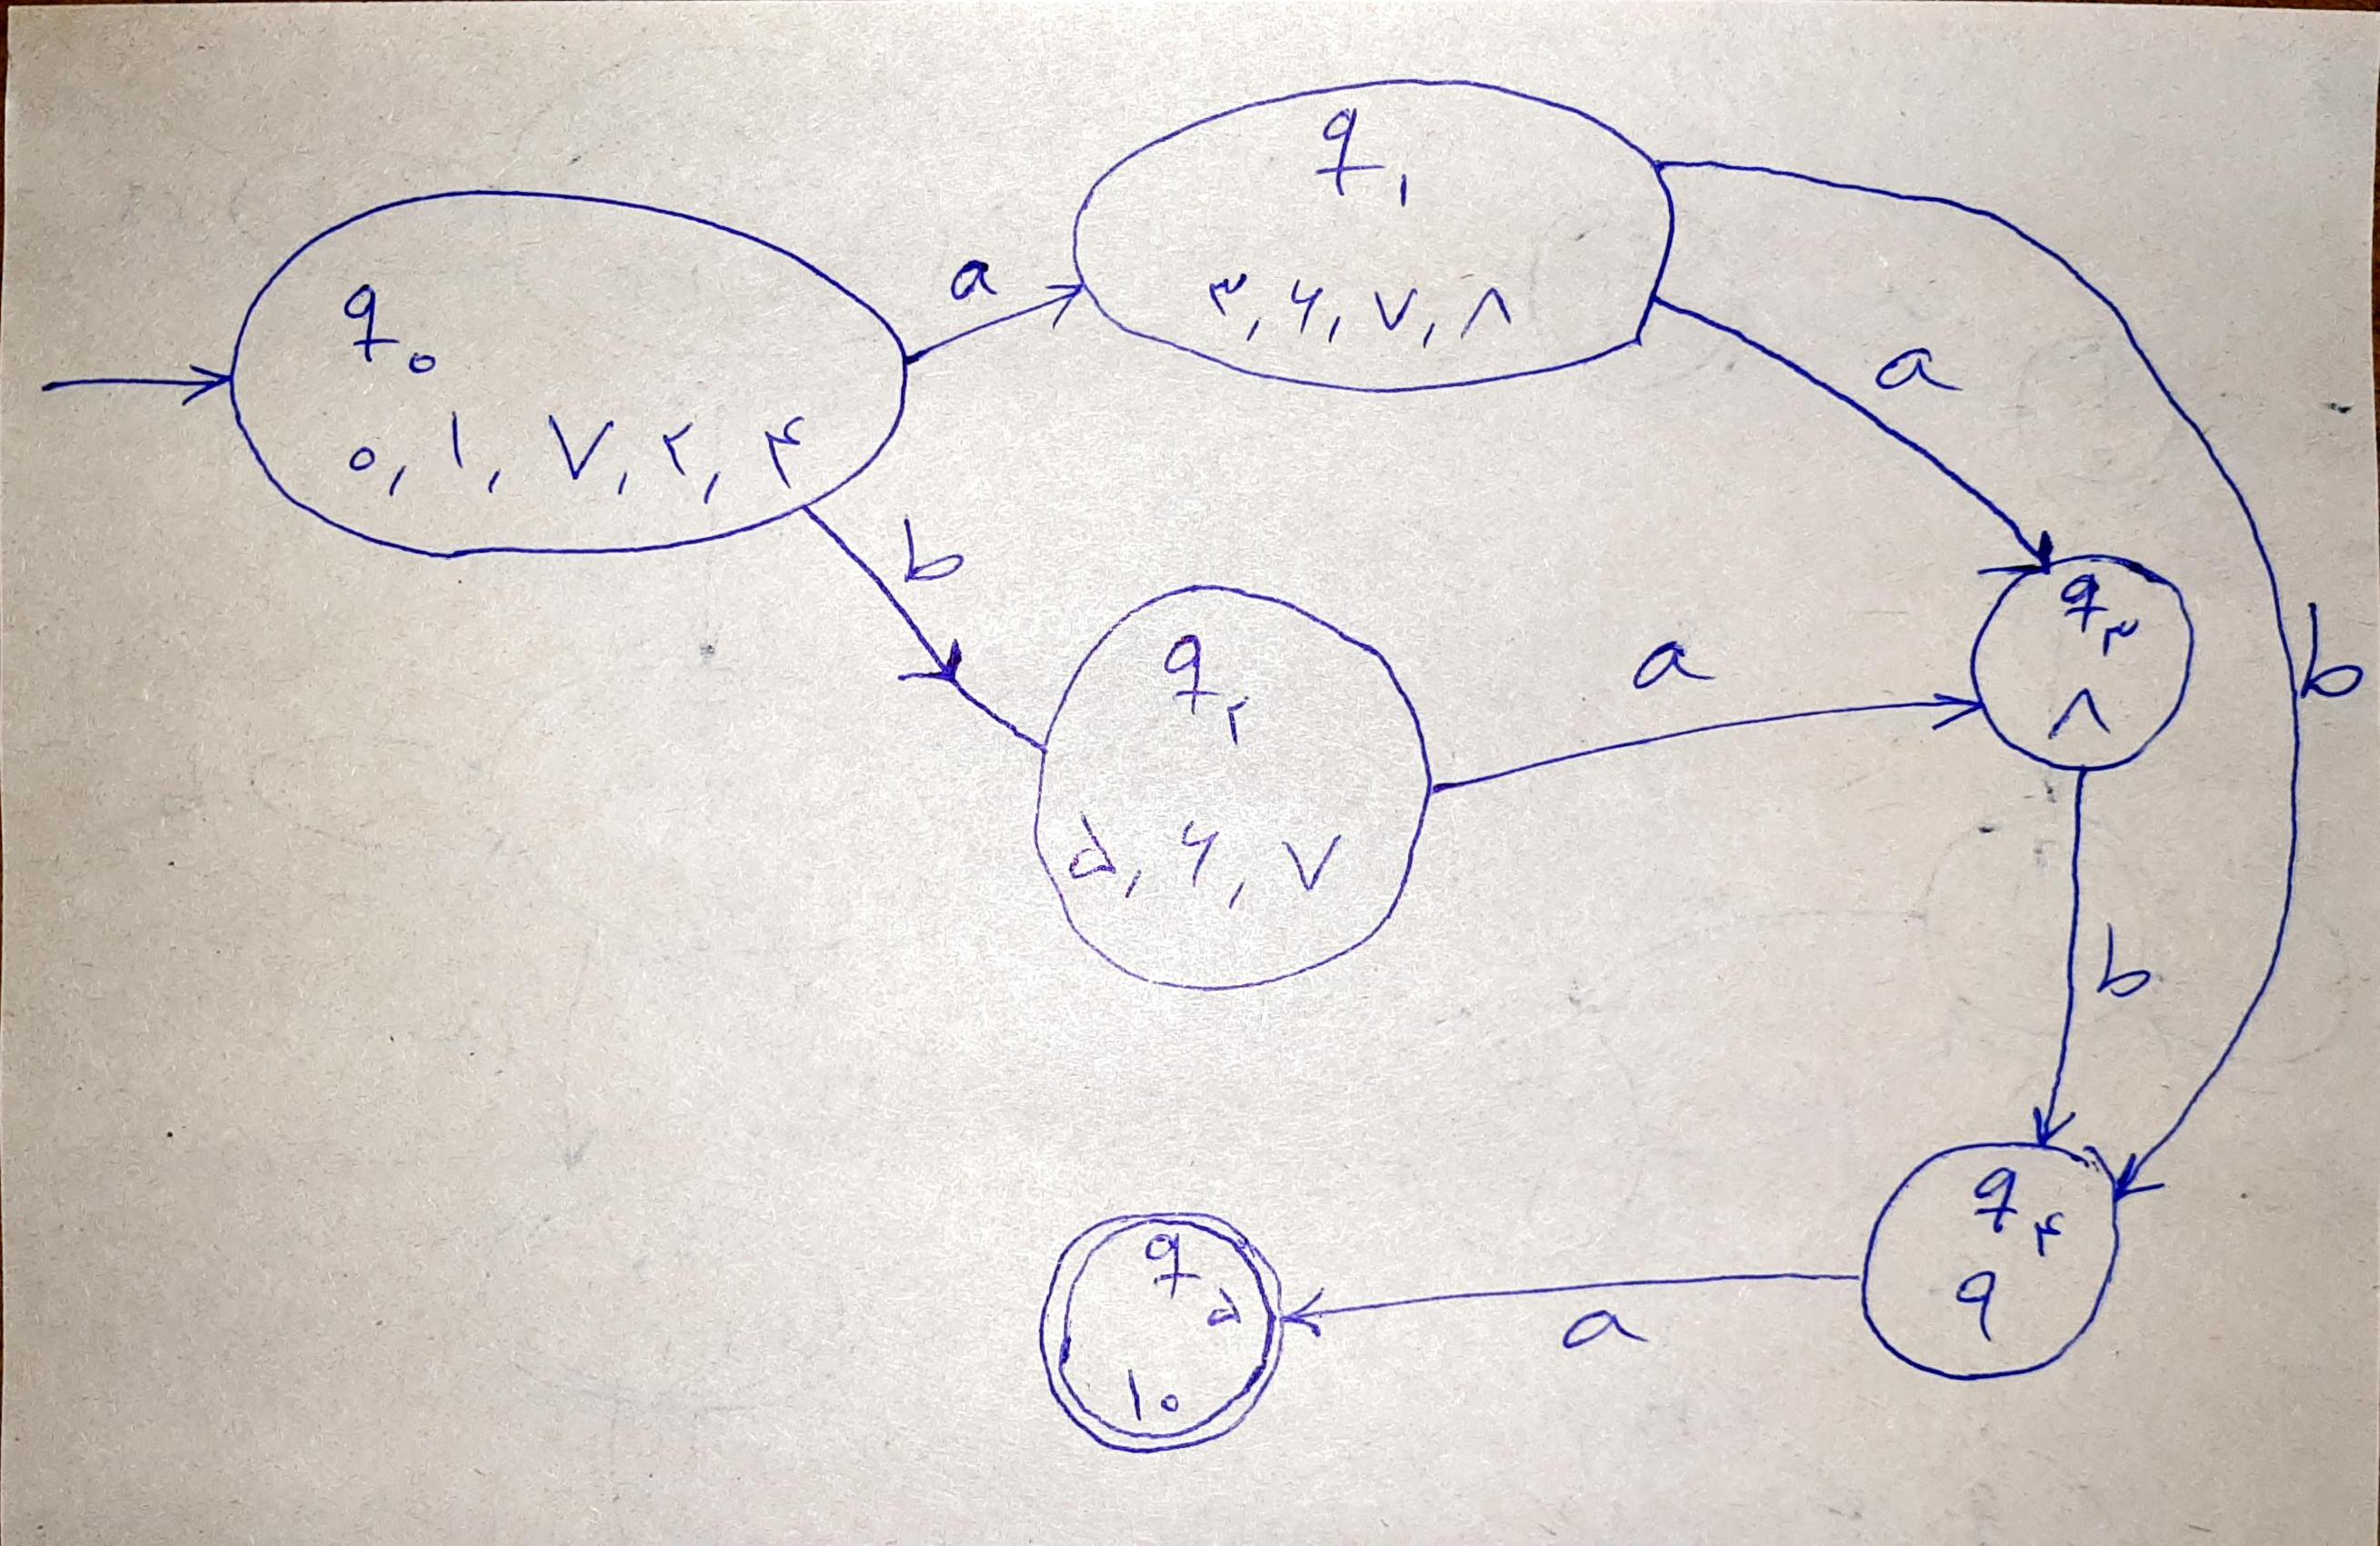
\includegraphics[width=1\textwidth]{figures/4a.jpg}
    \caption
	{}
    \label{fig:fig1}
\end{figure}
\subsection{ب}
\begin{figure}[H]
    \centering
    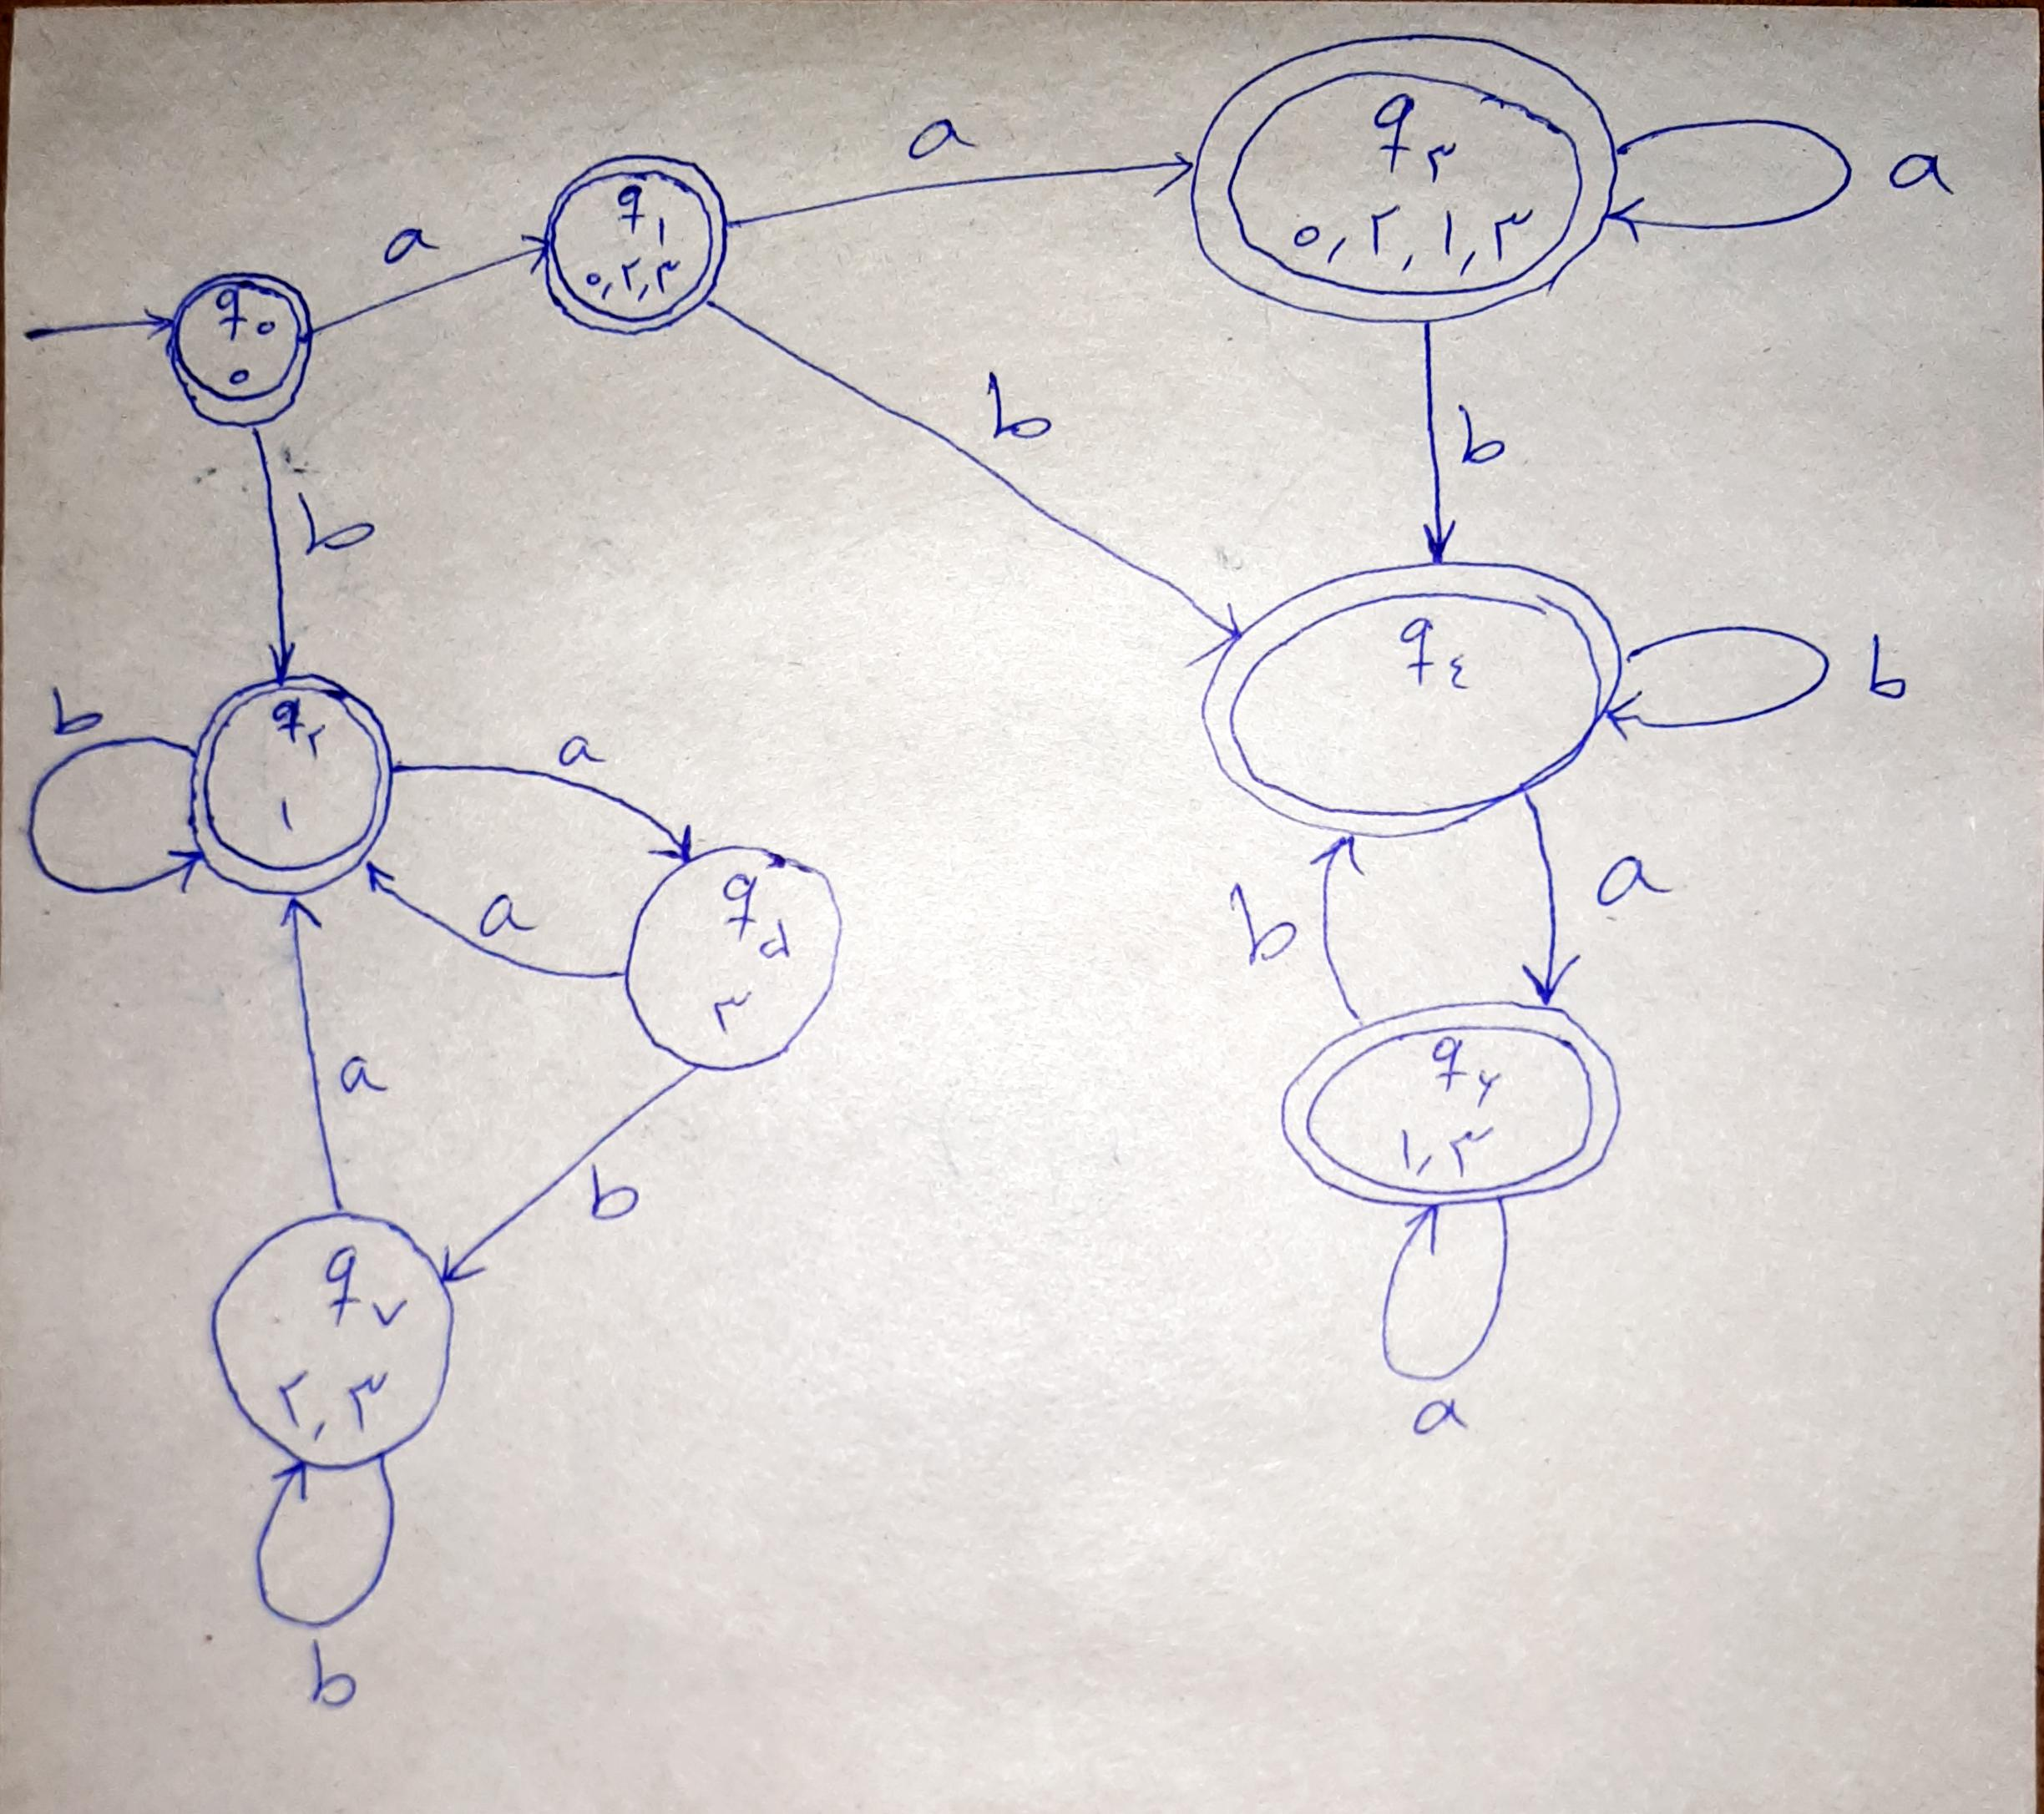
\includegraphics[width=1\textwidth]{figures/4b.jpg}
    \caption
	{}
    \label{fig:fig1}
\end{figure}


\section{}%5
\subsection{الف}
\begin{figure}[H]
    \centering
    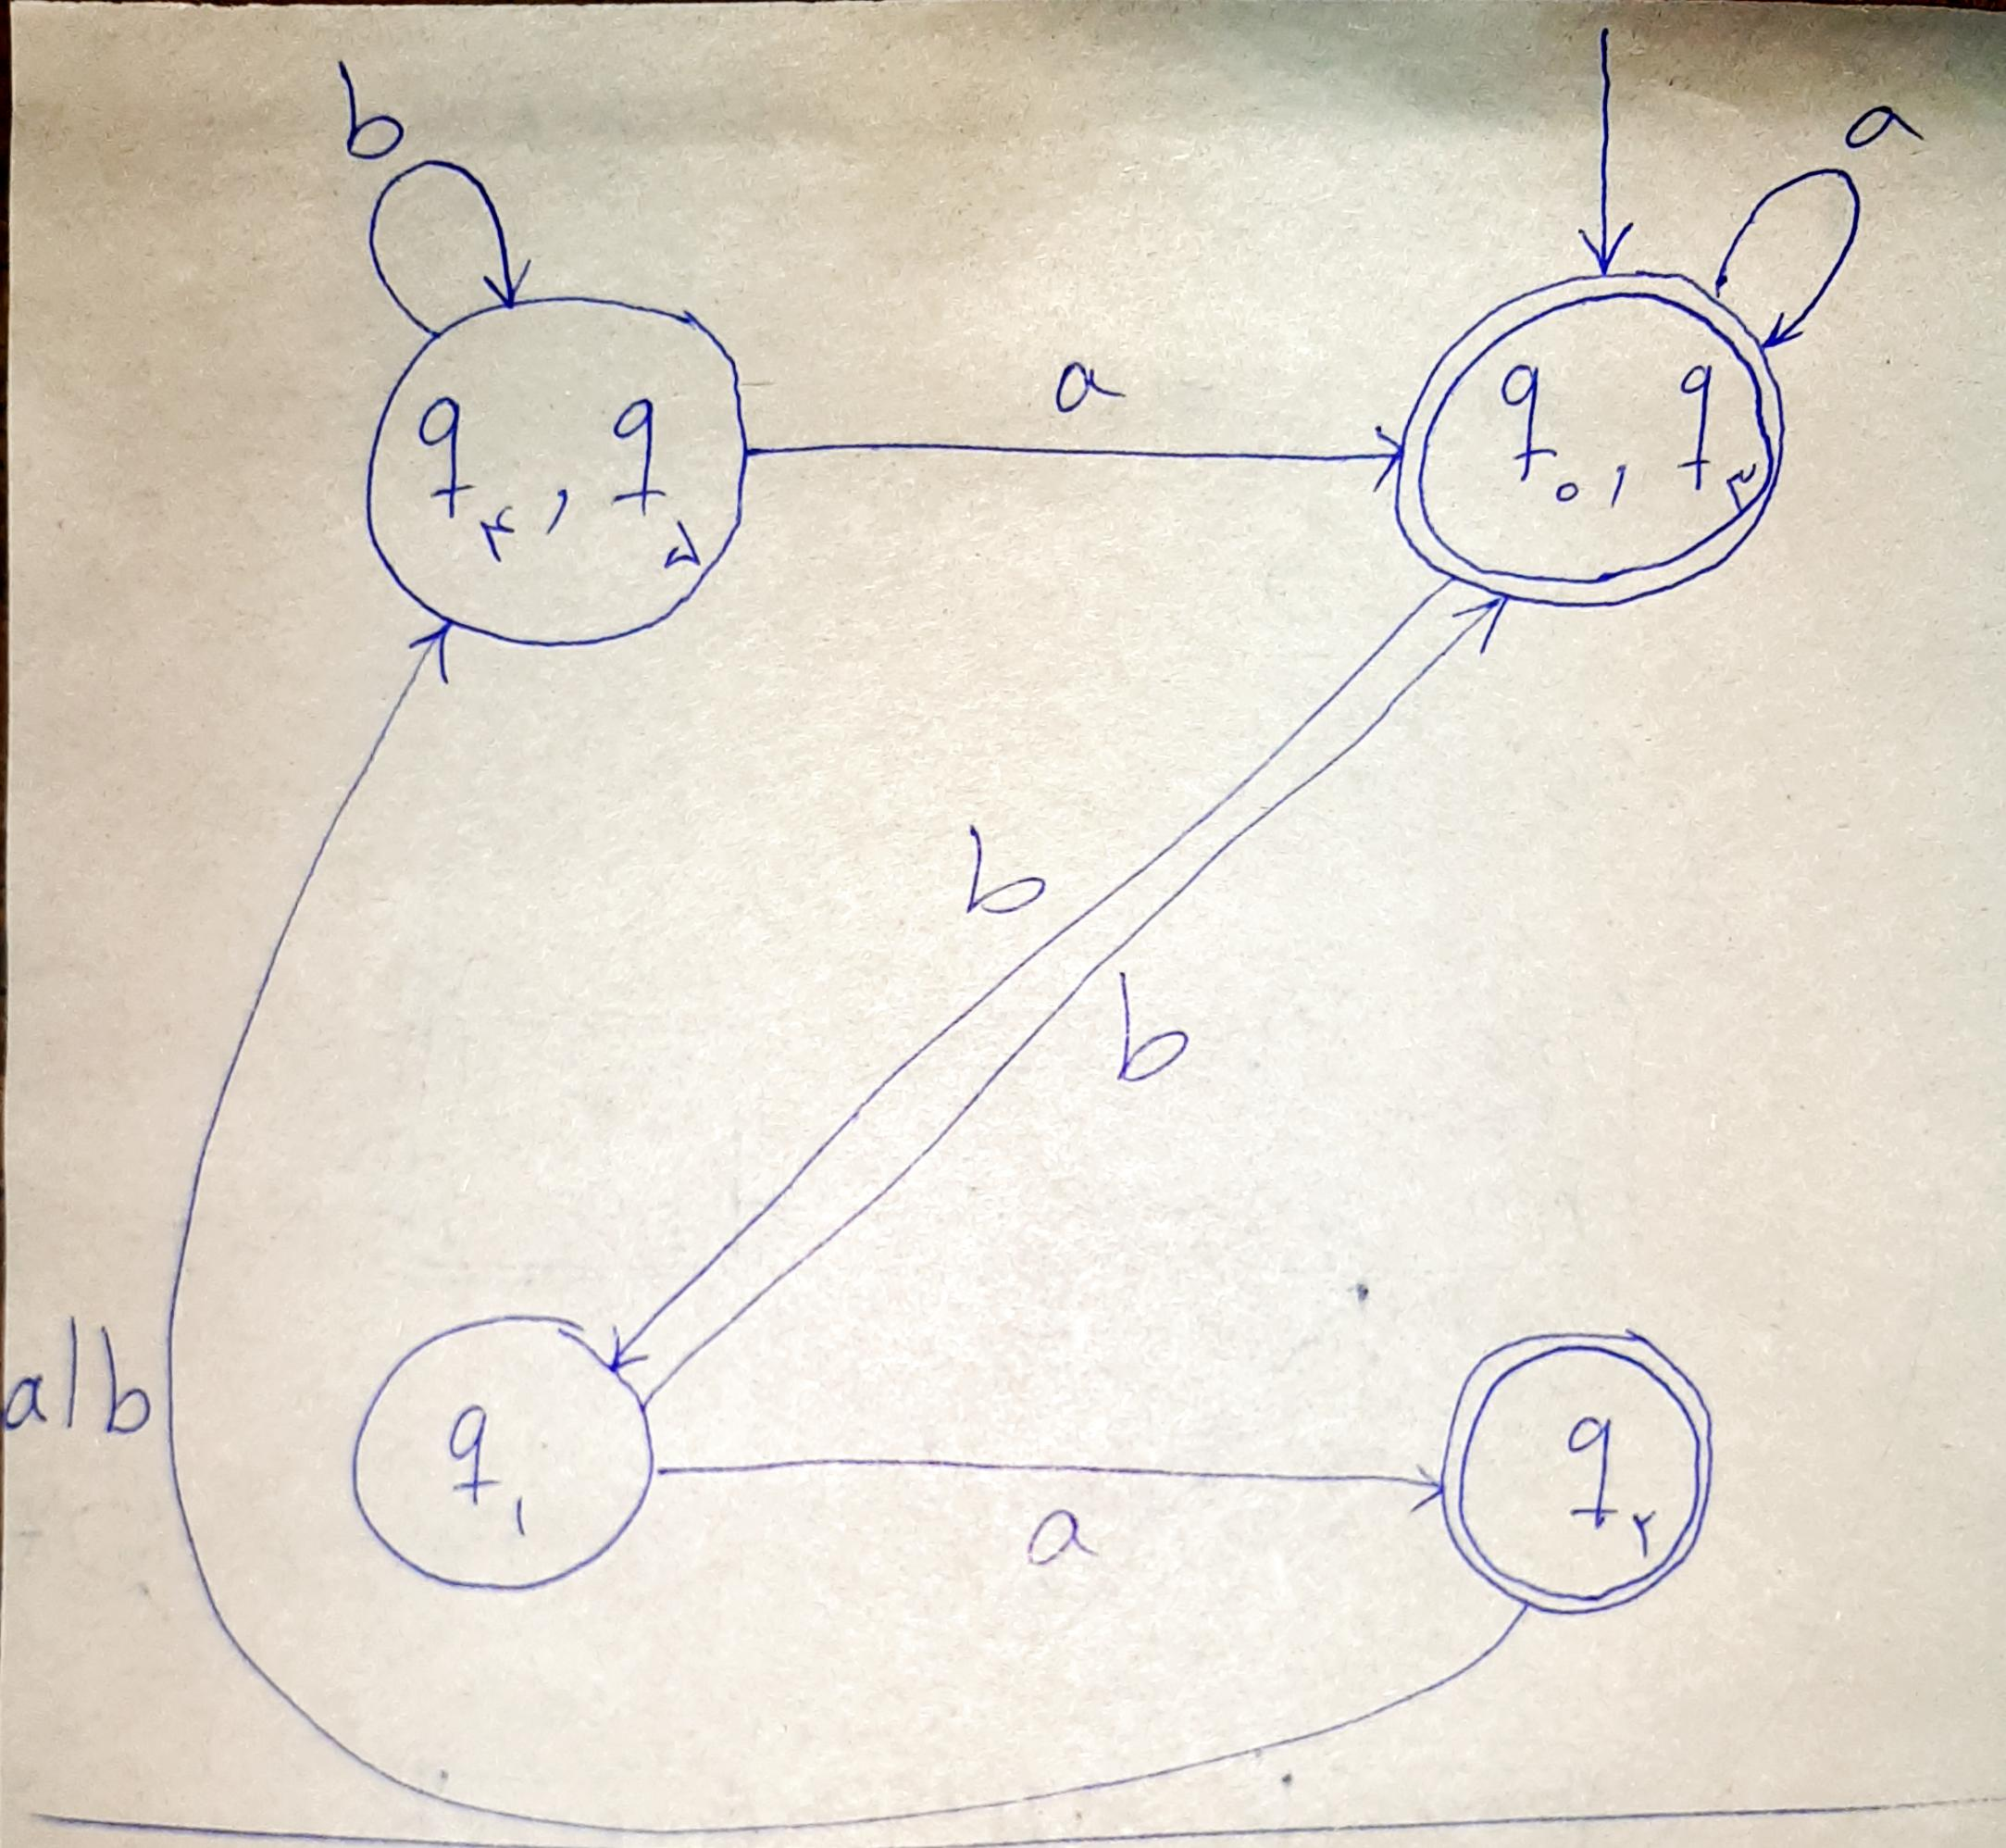
\includegraphics[width=1\textwidth]{figures/5a.jpg}
    \caption
	{}
    \label{fig:fig1}
\end{figure}
\subsection{ب}
قابل کمینه‌سازی نیست.

\section{}%6
\subsection{الف}
\begin{figure}[H]
    \centering
    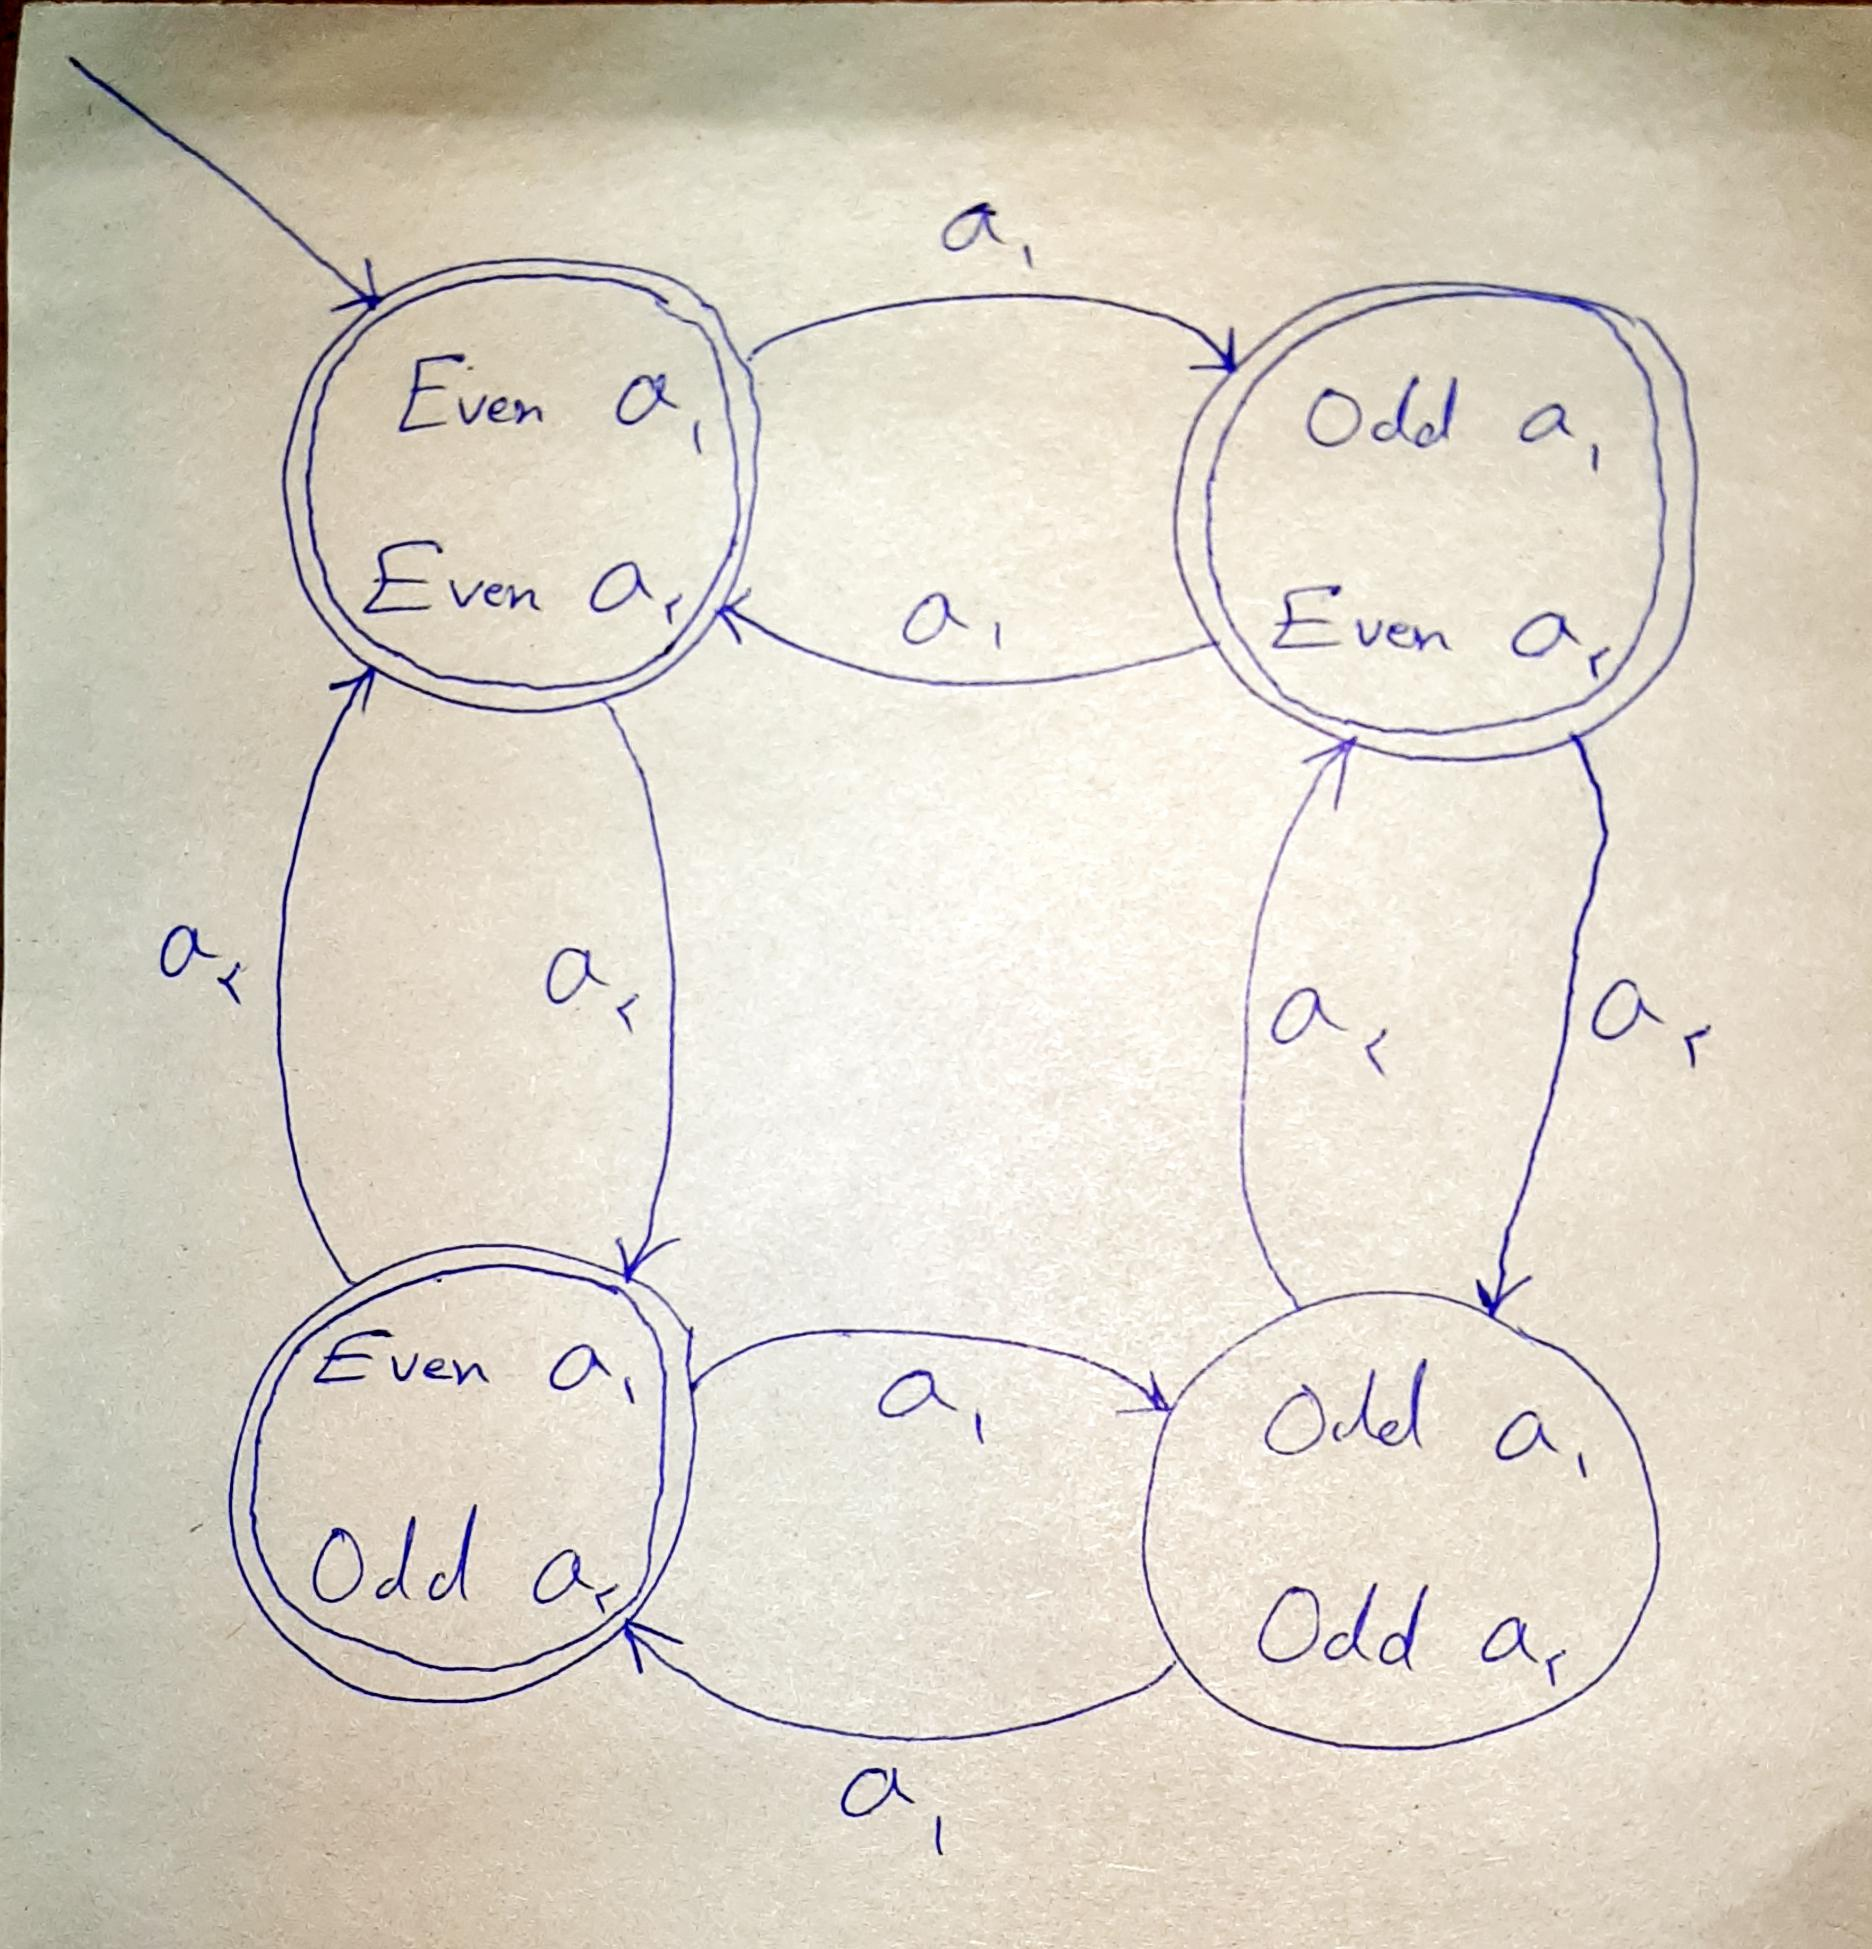
\includegraphics[width=1\textwidth]{figures/6a.jpg}
    \caption
	{}
    \label{fig:fig1}
\end{figure}
\subsection{ب}
\begin{figure}[H]
    \centering
    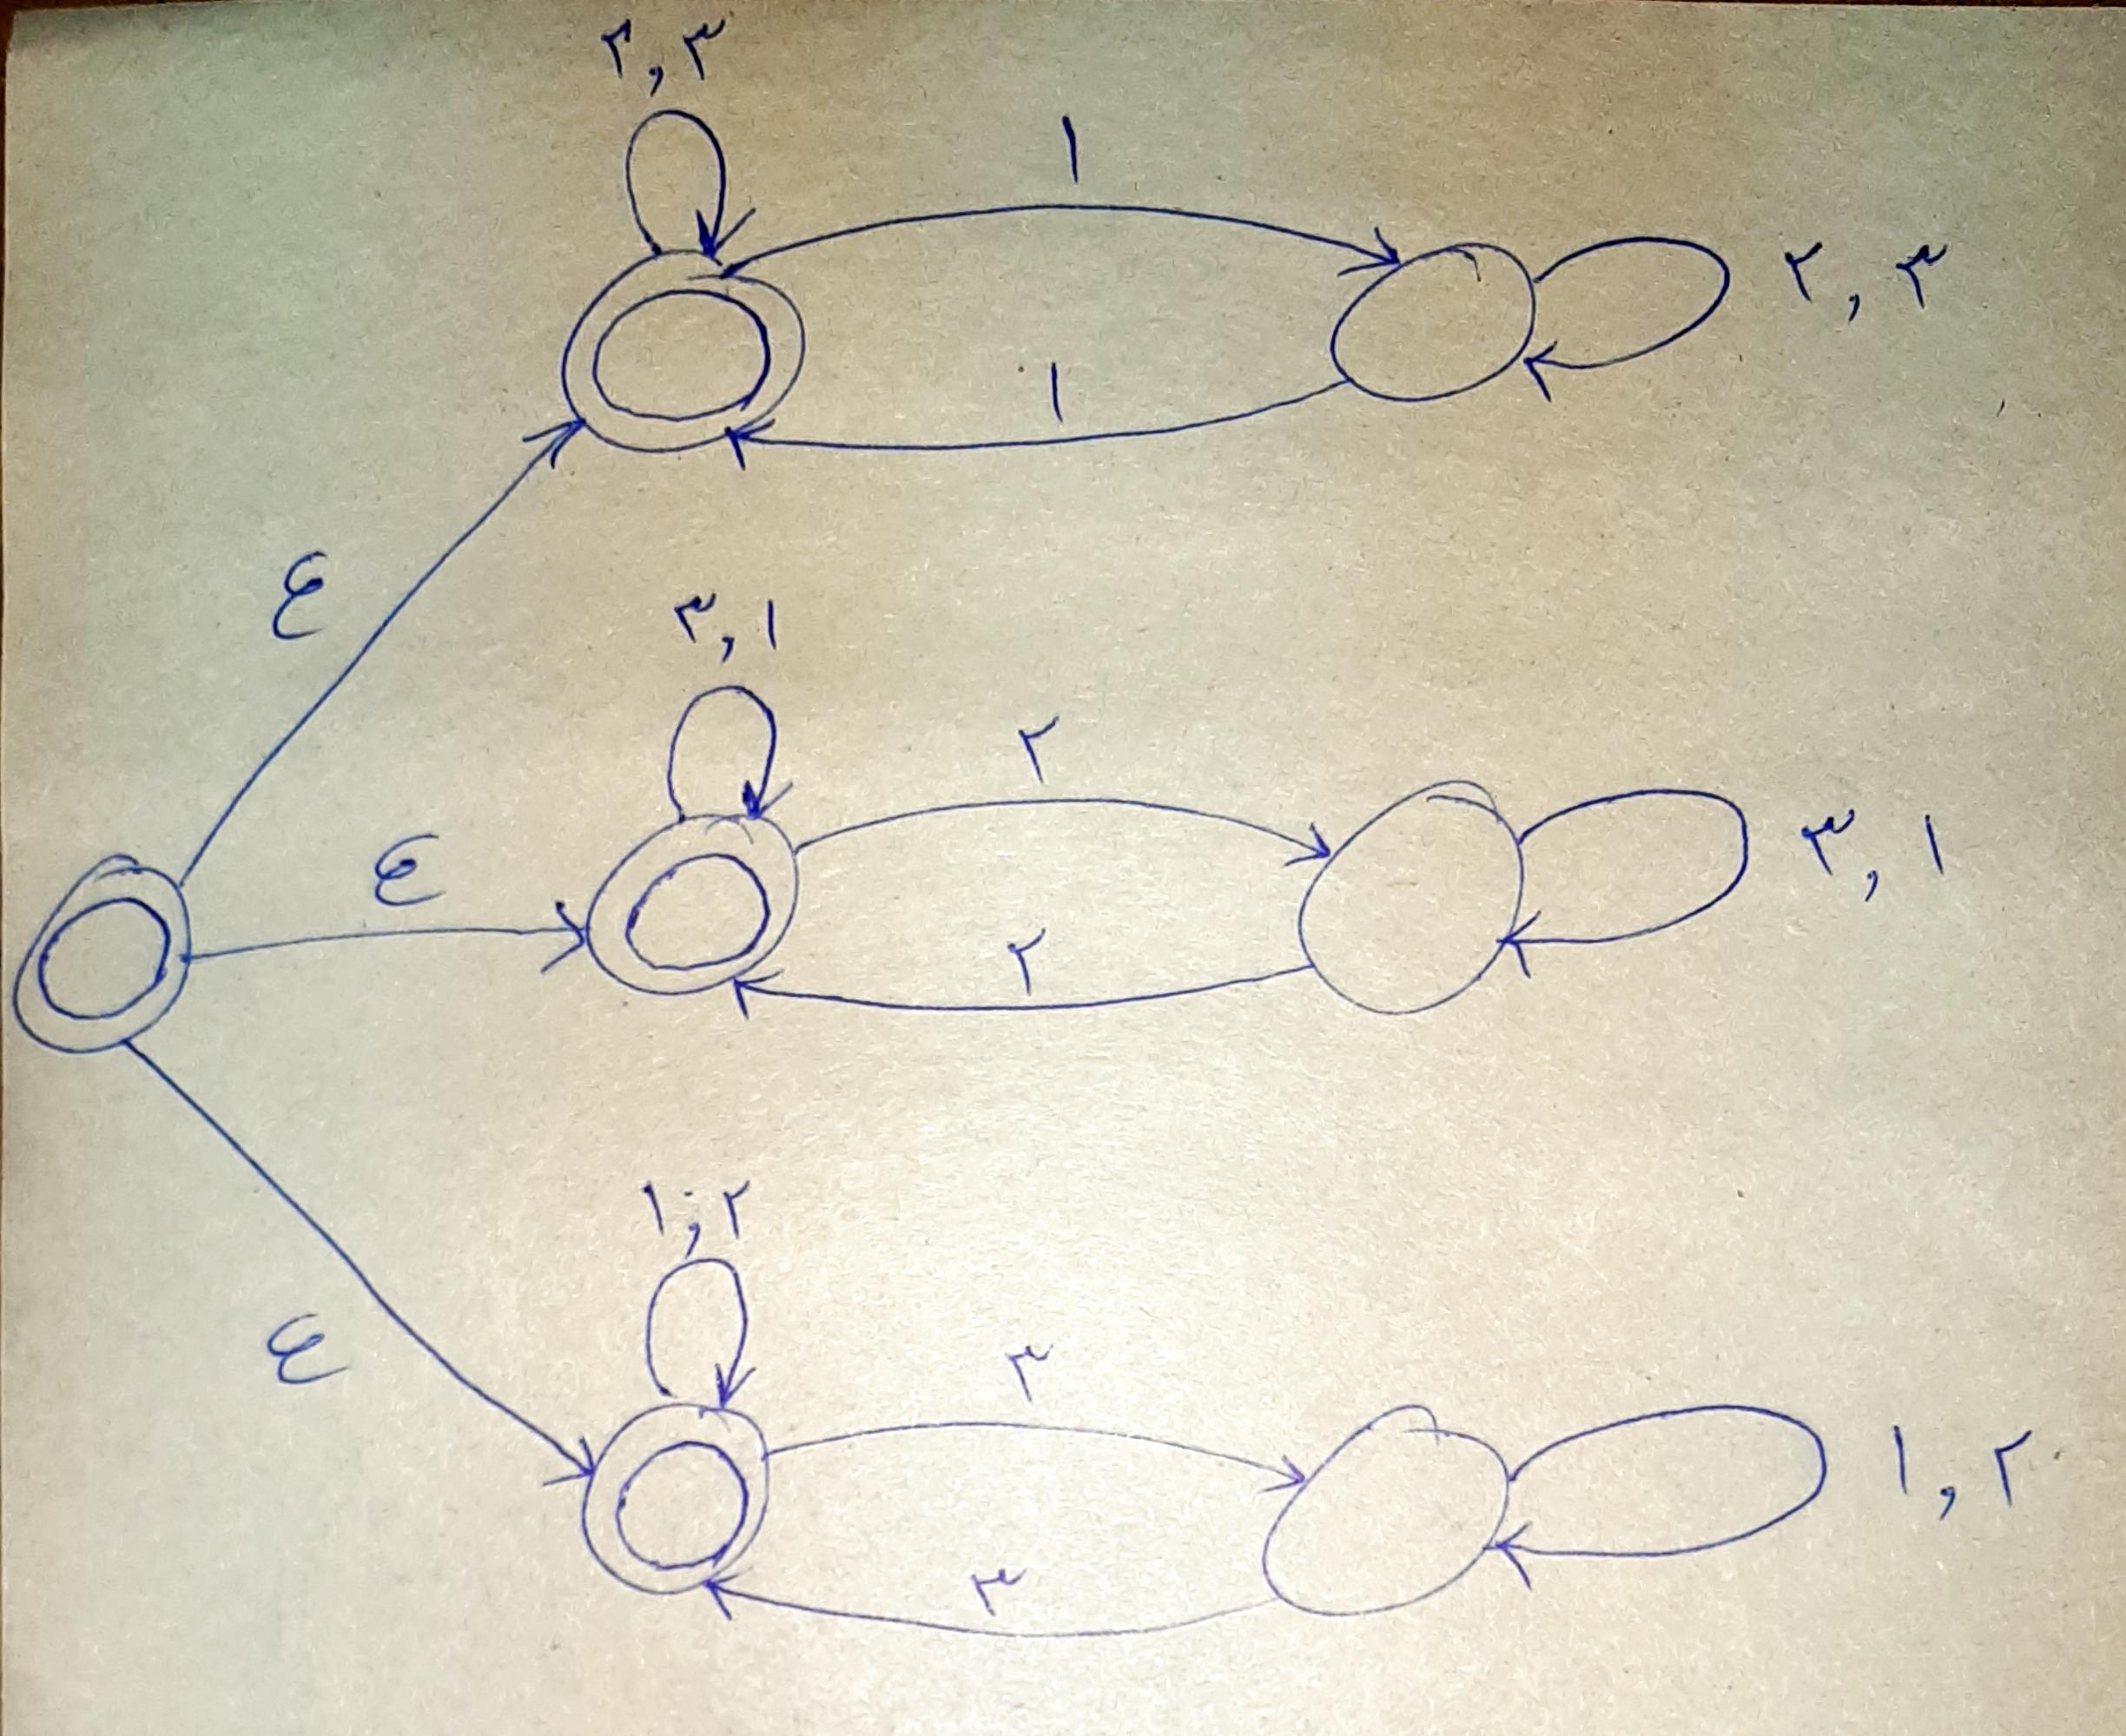
\includegraphics[width=1\textwidth]{figures/6b.jpg}
    \caption
	{}
    \label{fig:fig1}
\end{figure}



\section{}%7
\subsection{آ}
برای زوج بودن عبارتِ $2n_a\left( w \right) + 3n_b\left( w \right)$، $n_b\left( w \right)$ باید حتما زوج باشد. پس داریم:
\begin{latin}
$
\left( a \cup \left( bb \right) \right) ^ *
$
\end{latin}

\subsection{ب}
یا باید تعداد \lr{a}ها بزرگتر مساوی 3 باشد یا تعداد \lr{b}ها بزرگتر مساوی 2.
\begin{latin}
$
\left( aaa ^ + b ^ + \right) \cup \left( aa ^ + bb ^ + \right)
$
\end{latin}

\subsection{ج}
از آنجایی که $v$ تعداد حالات متناهی دارد هر یک از آن‌ها را به دست آورده و در نهایت اجتماع می‌گیریم.
\begin{latin}
$
a \left( a \cup b \right) ^ + a    \\
\cup    b \left( a \cup b \right) ^ + b    \\
\cup   aa \left( a \cup b \right) ^ + aa   \\
\cup   ab \left( a \cup b \right) ^ + ab   \\
\cup   ba \left( a \cup b \right) ^ + ba   \\
\cup   bb \left( a \cup b \right) ^ + bb   \\
\cup  aaa \left( a \cup b \right) ^ + aaa  \\
\cup  aab \left( a \cup b \right) ^ + aab  \\
\cup  aba \left( a \cup b \right) ^ + aba  \\
\cup  abb \left( a \cup b \right) ^ + abb  \\
\cup  baa \left( a \cup b \right) ^ + baa  \\
\cup  bab \left( a \cup b \right) ^ + bab  \\
\cup  bba \left( a \cup b \right) ^ + bba  \\
\cup  bbb \left( a \cup b \right) ^ + bbb  \\
\cup aaaa \left( a \cup b \right) ^ + aaaa \\
\cup aaab \left( a \cup b \right) ^ + aaab \\
\cup aaba \left( a \cup b \right) ^ + aaba \\
\cup aabb \left( a \cup b \right) ^ + aabb \\
\cup abaa \left( a \cup b \right) ^ + abaa \\
\cup abab \left( a \cup b \right) ^ + abab \\
\cup abba \left( a \cup b \right) ^ + abba \\
\cup abbb \left( a \cup b \right) ^ + abbb \\
\cup baaa \left( a \cup b \right) ^ + baaa \\
\cup baab \left( a \cup b \right) ^ + baab \\
\cup baba \left( a \cup b \right) ^ + baba \\
\cup babb \left( a \cup b \right) ^ + babb \\
\cup bbaa \left( a \cup b \right) ^ + bbaa \\
\cup bbab \left( a \cup b \right) ^ + bbab \\
\cup bbba \left( a \cup b \right) ^ + bbba \\
\cup bbbb \left( a \cup b \right) ^ + bbbb \\
$
\end{latin}

\subsection{د}
برای فرد بودن طول رشته‌ها باید زوجیت تعداد \lr{a}ها مخالف زوجیت تعداد \lr{b}ها باشد.
\begin{latin}
$
\left( aa \right) ^ * a \left( bb \right) ^ * \cup \left( aa \right) ^ * \left( bb \right) ^ * b
$
\end{latin}


\section{}%8
\subsection{}
\begin{latin}
\begin{longtable}[c]{|c|c|c|}
\hline
\textbf{\#} & \textbf{Token}          & \textbf{Type} \\ \hline
\textbf{1}  & main                    & ID            \\ \hline
\textbf{2}  & (                       & LPAREN        \\ \hline
\textbf{3}  & )                       & RPAREN        \\ \hline
\textbf{4}  & \{  					& LBRACE        \\ \hline
\textbf{5}  & int                     & INT           \\ \hline
\textbf{6}  & *                       & STAR          \\ \hline
\textbf{7}  & a                       & ID            \\ \hline
\textbf{8}  & ,                       & COMMA         \\ \hline
\textbf{9}  & b                       & ID            \\ \hline
\textbf{10} & ;                       & SEMI          \\ \hline
\textbf{11} & b                       & ID            \\ \hline
\textbf{12} & =                       & ASSIGNMENT    \\ \hline
\textbf{13} & 10                      & NUM           \\ \hline
\textbf{14} & ;                       & SEMI          \\ \hline
\textbf{15} & a                       & ID            \\ \hline
\textbf{16} & =                       & ASSIGNMENT    \\ \hline
\textbf{17} & \&                      & AMPERSAND     \\ \hline
\textbf{18} & b                       & ID            \\ \hline
\textbf{19} & ;                       & SEMI          \\ \hline
\textbf{20} & printf                  & ID            \\ \hline
\textbf{21} & (                       & LPAREN        \\ \hline
\textbf{22} & "\%d\%d"                & STRING        \\ \hline
\textbf{23} & ,                       & COMMA         \\ \hline
\textbf{24} & b                       & ID            \\ \hline
\textbf{25} & ,                       & COMMA         \\ \hline
\textbf{26} & *                       & STAR          \\ \hline
\textbf{27} & a                       & ID            \\ \hline
\textbf{28} & )                       & RPAREN        \\ \hline
\textbf{29} & ;                       & SEMI          \\ \hline
\textbf{30} & b                       & ID            \\ \hline
\textbf{31} & =                       & ASSIGNMENT    \\ \hline
\textbf{32} & *                       & STAR          \\ \hline
\textbf{33} & b                       & ID            \\ \hline
\textbf{34} & ;                       & SEMI          \\ \hline
\textbf{35} & \} & RBRACE      				  \\ \hline
\textbf{36} &                         & EOF           \\ \hline
\end{longtable}
\end{latin}

\subsection{}
\begin{latin}
\begin{longtable}[c]{|c|c|c|}
\hline
\textbf{\#} & \textbf{Token}            & \textbf{Type} \\ \hline
\textbf{1}  & main                      & ID            \\ \hline
\textbf{2}  & (                         & LPAREN        \\ \hline
\textbf{3}  & )                         & RPAREN        \\ \hline
\textbf{4}  & \{    & LBRACE        \\ \hline
\textbf{5}  & char                      & CHAR          \\ \hline
\textbf{6}  & ch                        & ID            \\ \hline
\textbf{7}  & =                         & ASSIGNMENT    \\ \hline
\textbf{8}  & 'A'                       & CHARACTER     \\ \hline
\textbf{9}  & ;                         & SEMI          \\ \hline
\textbf{10} & int                       & INT           \\ \hline
\textbf{11} & x                         & ID            \\ \hline
\textbf{12} & ,                         & COMMA         \\ \hline
\textbf{13} & y                         & ID            \\ \hline
\textbf{14} & ;                         & SEMI          \\ \hline
\textbf{15} & x                         & ID            \\ \hline
\textbf{16} & =                         & ASSIGNMENT    \\ \hline
\textbf{17} & y                         & ID            \\ \hline
\textbf{18} & =                         & ASSIGNMENT    \\ \hline
\textbf{19} & 20                        & NUM           \\ \hline
\textbf{20} & ;                         & SEMI          \\ \hline
\textbf{21} & x                         & ID            \\ \hline
\textbf{22} & ++                        & INCREMENT     \\ \hline
\textbf{23} & ;                         & SEMI          \\ \hline
\textbf{24} & printf                    & ID            \\ \hline
\textbf{25} & (                         & LPAREN        \\ \hline
\textbf{26} & "\%d\%\:d" & STRING        \\ \hline
\textbf{27} & ,                         & COMMA         \\ \hline
\textbf{28} & x                         & ID            \\ \hline
\textbf{29} & ,                         & COMMA         \\ \hline
\textbf{30} & y                         & ID            \\ \hline
\textbf{31} & )                         & RPAREN        \\ \hline
\textbf{32} & ;                         & SEMI          \\ \hline
\textbf{33} & \}   & RBRACE        \\ \hline
\textbf{34} &                           & EOF           \\ \hline
\end{longtable}
\end{latin}

\subsection{}
\begin{latin}
% Please add the following required packages to your document preamble:
% \usepackage{longtable}
% Note: It may be necessary to compile the document several times to get a multi-page table to line up properly
\begin{longtable}[c]{|c|c|c|}
\hline
\textbf{\#} & \textbf{Token}          & \textbf{Type}         \\ \hline
\textbf{1}  & int                     & INT                   \\ \hline
\textbf{2}  & strange                 & ID                    \\ \hline
\textbf{3}  & (                       & LPAREN                \\ \hline
\textbf{4}  & int                     & INT                   \\ \hline
\textbf{5}  & x                       & ID                    \\ \hline
\textbf{6}  & )                       & RPAREN                \\ \hline
\textbf{7}  & \{  & LBRACE                \\ \hline
\textbf{8}  & if                      & IF                    \\ \hline
\textbf{9}  & (                       & LPAREN                \\ \hline
\textbf{10} & x                       & ID                    \\ \hline
\textbf{11} & \textless{}=            & LESS THAN OR EQUAL TO \\ \hline
\textbf{12} & 0                       & NUM                   \\ \hline
\textbf{13} & )                       & RPAREN                \\ \hline
\textbf{14} & return                  & RETURN                \\ \hline
\textbf{15} & 0                       & NUM                   \\ \hline
\textbf{16} & ;                       & SEMI                  \\ \hline
\textbf{17} & if                      & IF                    \\ \hline
\textbf{18} & (                       & LPAREN                \\ \hline
\textbf{19} & (                       & LPAREN                \\ \hline
\textbf{20} & x                       & ID                    \\ \hline
\textbf{21} & \%                      & MODULUS               \\ \hline
\textbf{22} & 2                       & NUM                   \\ \hline
\textbf{23} & )                       & RPAREN                \\ \hline
\textbf{24} & !=                      & NOTEQ                 \\ \hline
\textbf{25} & 0                       & NUM                   \\ \hline
\textbf{26} & )                       & RPAREN                \\ \hline
\textbf{27} & return                  & RETURN                \\ \hline
\textbf{28} & x                       & ID                    \\ \hline
\textbf{29} & -                       & SUBTRACTION           \\ \hline
\textbf{30} & 1                       & NUM                   \\ \hline
\textbf{31} & ;                       & SEMI                  \\ \hline
\textbf{32} & return                  & RETURN                \\ \hline
\textbf{33} & 1                       & NUM                   \\ \hline
\textbf{34} & +                       & ADDITION              \\ \hline
\textbf{35} & strange                 & ID                    \\ \hline
\textbf{36} & (                       & LPAREN                \\ \hline
\textbf{37} & x                       & ID                    \\ \hline
\textbf{38} & -                       & SUBTRACTION           \\ \hline
\textbf{39} & 1                       & NUM                   \\ \hline
\textbf{40} & )                       & RPAREN                \\ \hline
\textbf{41} & ;                       & SEMI                  \\ \hline
\textbf{42} & \} & RBRACE                \\ \hline
\textbf{43} &                         & EOF                   \\ \hline
\end{longtable}
\end{latin}








%%%%%%%%%%%%%%%%%%%%%%%%%%%%%%%%%%%%%%%%%%%%%%%%%%%%%%%%%%%%%%%%%%%%%%

%\begin{latin}
%\lstinputlisting{sources/p2.m}
%\end{latin}


%%%%%%%%%%%%%%%%%%%%%%%%%%%%%%%%%%%
%%%%%%%%%%%%%%%%%%%%%%%%%%%%%%%%%%%
%%%%%%%%%%%%%%%%%%%%%%%%%%%%%%%%%%%

%------------------------------------------------------------------------------------------


\subsection*{منابع}
\renewcommand{\subsection}[2]{}%
\begin{thebibliography}{99} % assumes less than 100 references
%چنانچه مرجع فارسی نیز داشته باشید باید دستور فوق را فعال کنید و مراجع فارسی خود را بعد از این دستور وارد کنید


\begin{LTRitems}

\resetlatinfont

\bibitem{b1}
\end{LTRitems}

\end{thebibliography}


\end{document}
